% Три пути через поворот: хорда, дуга и касательная — русское издание.
% Перевод статьи «Three Ways Across a Turn: Chord, Arc and Tangent» (doi:10.5281/zenodo.24375338).
% Сборка: xelatex paper_ru.tex (дважды). Текст по частям: part1.tex … part5.tex.
\documentclass[11pt]{article}
\usepackage[margin=1.1in,headsep=18pt]{geometry}
\newcommand{\dgshorttitle}{Три пути через поворот}
\newcommand{\dgauthorshort}{Б. Р. Дэвис}
\usepackage{graphicx}
\graphicspath{{./}{../}}
\usepackage{float}
\usepackage{amsmath,amsthm}
% Davis Geometric house style, XeLaTeX edition for Russian (Cyrillic) text.
% Same layout as dgstyle.tex; text in Palatino (system font, with Cyrillic) through fontspec,
% math in newpxmath, Russian hyphenation and conventions through babel.
% Loaded with \input{../dgstyle} after amsmath and amsthm (do not load amssymb: newpxmath provides it).
% Needs (TeX Live): newpx, titlesec, caption, fancyhdr, microtype, xcolor, enumitem.
\usepackage[slantedGreek]{newpxmath}
\usepackage[no-math]{fontspec}
\setmainfont{Palatino}
\setsansfont{PT Sans}
\setmonofont{Menlo}[Scale=0.86]
\usepackage[english,russian]{babel}   % babel, not polyglossia: polyglossia rejects the macOS Palatino's script tags
\linespread{1.06}
\usepackage{microtype}
\usepackage{xcolor}
\definecolor{dgink}{HTML}{1F2328}
\definecolor{dgmuted}{HTML}{5A5F66}
\definecolor{dgrule}{HTML}{C9CDD2}
\definecolor{dgchord}{HTML}{2A78D6}
\definecolor{dgarc}{HTML}{1BAF7A}
\definecolor{dgtan}{HTML}{EB6834}
\definecolor{dgblend}{HTML}{6250D6}
% headings: numbered small caps, quiet rules of space rather than ink
\usepackage{titlesec}
\titleformat{\section}{\normalfont\large\bfseries\color{dgink}}{\thesection}{1em}{}  % no Cyrillic small caps in Palatino
\titleformat{\subsection}{\normalfont\normalsize\itshape\color{dgink}}{\thesubsection}{0.8em}{}
\titleformat{\subsubsection}[runin]{\normalfont\normalsize\itshape}{\thesubsubsection}{0.6em}{}[.]
\titleformat{\paragraph}[runin]{\normalfont\normalsize\itshape}{}{0pt}{}  % sources end paragraph titles with their own stop
\titlespacing*{\section}{0pt}{2.4ex plus 0.6ex minus 0.3ex}{1.1ex plus 0.2ex}
\titlespacing*{\subsection}{0pt}{1.8ex plus 0.5ex minus 0.2ex}{0.7ex plus 0.2ex}
\titlespacing*{\paragraph}{0pt}{1.2ex plus 0.4ex minus 0.2ex}{0.6em}
% captions: small, label in small caps, ragged
\usepackage[font=small,labelfont=bf,labelsep=period,justification=justified,margin=4pt]{caption}
% running heads
\usepackage{fancyhdr}
\pagestyle{fancy}
\fancyhf{}
\renewcommand{\headrulewidth}{0pt}
\fancyhead[L]{\small\color{dgmuted}\dgauthorshort}
\fancyhead[R]{\small\itshape\color{dgmuted}\dgshorttitle}
\fancyfoot[C]{\small\color{dgmuted}\thepage}
\fancypagestyle{plain}{\fancyhf{}\fancyfoot[C]{\small\color{dgmuted}\thepage}}
\setlength{\headheight}{14pt}
% title block
\makeatletter
\renewcommand{\maketitle}{%
  \thispagestyle{plain}%
  \begin{center}
    {\LARGE\color{dgink}\@title\par}\vspace{1.1em}
    {\large\@author\par}\vspace{0.5em}
    {\small\color{dgmuted}\@date\par}
  \end{center}\vspace{0.6em}}
\renewenvironment{abstract}{%
  \begin{list}{}{\setlength{\leftmargin}{2.2em}\setlength{\rightmargin}{2.2em}}\item\relax
  \small\noindent{\bfseries Аннотация.}\enspace}{\end{list}\vspace{0.4em}}
\makeatother
\usepackage{enumitem}
\setlist{itemsep=0.25ex, topsep=0.6ex}
% "In plain words": a quiet ruled aside
\newenvironment{plain}{%
  \par\smallskip\begin{list}{}{\setlength{\leftmargin}{1.4em}\setlength{\rightmargin}{1.4em}}\item\relax
  \small\color{dgink}\noindent{\itshape Простыми словами.}\enspace}{\end{list}\smallskip}

\usepackage{booktabs}
\usepackage{tikz}
\usepackage[hidelinks]{hyperref}
\usepackage{url}
\expandafter\def\expandafter\UrlBreaks\expandafter{\UrlBreaks\do\_\do\-}
\setlength{\emergencystretch}{2.5em}   % long Russian words
\usepackage{listings}
\usepackage{array}
\lstdefinestyle{rust}{basicstyle=\ttfamily\footnotesize, columns=fullflexible, keepspaces=true,
  frame=lines, framesep=4pt, xleftmargin=6pt, xrightmargin=6pt, showstringspaces=false,
  morekeywords={let,mut,for,in,fn,pub}}

\newtheorem{proposition}{Предложение}
\newtheorem{remark}{Замечание}

\title{Три пути через поворот:\\ хорда, дуга и касательная}
\author{Би Роза Дэвис\\[1pt] {\normalsize\upshape\itshape Davis Geometric}}
\date{Ноябрь 2026}

\begin{document}
\maketitle

\begin{abstract}
Когда единичный отрезок поворачивается на угол $\theta$, его конец можно соединить с
исходным положением тремя естественными способами: прямой хордой, дугой, которую
действительно описывает поворот, и двумя касательными, пересекающимися вне окружности.
Их длины равны $2\sin(\theta/2)$, $\theta$ и $2\tan(\theta/2)$, и они всегда идут именно в
этом порядке. Всё это классика, от Архимеда до Снеллиуса и Гюйгенса. В настоящей работе
собрано, что означают эти три пути, если поворот рассматривать как комплексное число
$U=e^{i\theta}$ или как единичный кватернион. Хорда есть $U-1$, и её квадрат~--- энергия
Вильсона на решётке. Дуга есть логарифм, и её квадрат~--- энергия континуума. Отрезок
касательной $\tan(\theta/2)$ есть параметр Кэли, из которого $U$ строится алгебраически, а
если читать его как шаг по времени, он даёт метод Кранка~--- Николсон. Хорда и касательная
отклоняются от дуги в противоположные стороны, причём касательная в главном порядке ровно
вдвое сильнее. Поэтому веса Снеллиуса~--- Гюйгенса
$2{:}1$ уничтожают главную ошибку как в длине, так и в энергии: $(2C^2+T^2)/3=\theta^2+
\tfrac{7}{720}\theta^6+\dots$. Половина хорды есть расстояние $d$ из тождества $S+d^2=1$,
где сходство $S=\cos^2(\theta/2)$. На сетках $SU(2)$ из нашей работы о восстановлении
кривизны углы граней достаточно малы (не более $0.094$), так что энергии хорды и дуги
различаются менее чем на $0.08\%$; следовательно, эти поправки не являются источником
измеренных там ошибок.
У каждого промаха есть близнец с другой стороны, а при пересечении границы окружности
поворот становится мнимым, тогда как $S+d^2=1$ сохраняется. Парадокс Бертрана оказывается
вопросом о том, какая из этих величин считается равномерно распределённой: дуга, $\sqrt S$ или $S$.
Игра в билеты помещает всё это в одну комнату: дуга, хорда и энергия покупают по одному билету каждая при своём угле ($57.30^\circ$, $60^\circ$, $90^\circ$), а на два целых билета повернуться можно только в центре или в его близнеце.
Каждое тождество проверено символьно или численно скриптом, прилагаемым к статье.
В калибровочном поле каждая малая петля несёт поворот~--- свою голономию, и картина
читается напрямую: поворот создаёт энергию, решётка оплачивает её по хорде, а наименьшая
единица поворота искривлена просто потому, что она существует. В сопутствующей работе
вычисления с этими поворотами проводятся на гомологической сфере Пуанкаре.
\end{abstract}

\section{Картинка}\label{sec:picture}

Проведём отрезок длины один из начала координат в точку $1$. Повернём его на угол
$\theta$. Его конец движется по единичной окружности из $1$ в $e^{i\theta}$. Если
поворачивать его во всех направлениях, конец опишет всю окружность.

Теперь попросим два положения конца снова встретиться. Есть три естественных способа
(рис.~\ref{fig:three}). \emph{Хорда} идёт прямо сквозь круг. \emph{Дуга} идёт по
окружности, тем же путём, что и поворот. \emph{Внешний путь} идёт по касательной в одном
конце до точки, где она пересекается с касательной в другом конце, а затем возвращается
внутрь. Дуга~--- единственный из трёх путей, по которому может пройти сам поворот; хорда~---
короткий путь напрямик, срезающий поперёк, а внешний путь~--- обход, который в промежутке
нигде не касается окружности.

\begin{plain}
Если повернуть палочку на какой-то угол, её кончик пройдёт по кривой. После этого два
положения кончика можно соединить: срезать напрямик (хорда), пройти по кругу тем же путём,
что и палочка (дуга), или выйти наружу по двум боковым линиям и вернуться (внешний путь).
Путь напрямик всегда самый короткий, обход всегда самый длинный. Истинный путь лежит между ними.
Эта статья о том, что означает каждый из трёх путей и чего он стоит.
\end{plain}

\begin{figure}[t]\centering
\begin{tikzpicture}[scale=3.2]
  \def\t{70}
  \draw[gray!60] (0,0) circle (1);
  \draw[->,gray] (-1.15,0) -- (1.5,0);
  \draw[->,gray] (0,-0.3) -- (0,1.25);
  \draw[thick] (0,0) -- (1,0);
  \draw[thick] (0,0) -- ({cos(\t)},{sin(\t)});
  \draw[very thick,dgarc] (1,0) arc (0:\t:1);
  \draw[very thick,dgchord] (1,0) -- ({cos(\t)},{sin(\t)});
  \coordinate (Q) at ({1/cos(\t/2)*cos(\t/2)},{1/cos(\t/2)*sin(\t/2)});
  \draw[very thick,dgtan] (1,0) -- (Q) -- ({cos(\t)},{sin(\t)});
  \draw (0.22,0) arc (0:\t:0.22); \node at ({0.3*cos(\t/2)},{0.3*sin(\t/2)}) {$\theta$};
  \fill (1,0) circle (0.02) node[below right] {$1$};
  \fill ({cos(\t)},{sin(\t)}) circle (0.02) node[above] {$U=e^{i\theta}$};
  \node[dgchord] at (0.62,0.30) {хорда};
  \node[dgarc] at (0.80,0.47) {дуга};
  \node[dgtan] at (1.26,0.80) {внешний};
\end{tikzpicture}
\caption{Три пути через поворот на $\theta=70^\circ$: хорда (длина $2\sin(\theta/2)$),
дуга ($\theta$) и внешний путь по двум касательным ($2\tan(\theta/2)$).}
\label{fig:three}
\end{figure}

Обозначим три длины через $C=2\sin(\theta/2)$, $A=\theta$ и $T=2\tan(\theta/2)$. Внешняя
вершина лежит на биссектрисе на расстоянии $\sec(\theta/2)$ от центра, поэтому каждый
отрезок касательной имеет длину $\tan(\theta/2)$. На рис.~\ref{fig:sphere} те же три
пути изображены в пространстве, на сфере, где живут неабелевы повороты из раздела~\ref{sec:su2}.

\begin{figure}[t]\centering
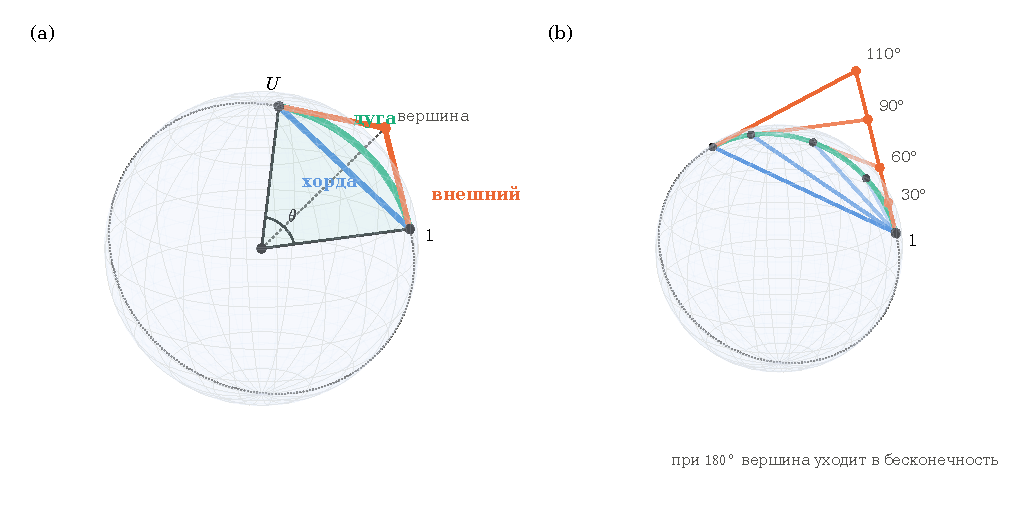
\includegraphics[width=\linewidth]{figures/fig_sphere_3d.pdf}
\caption{Три пути в трёх измерениях. \textbf{(a)} Поворот на $\theta=70^\circ$ в плоскости,
проходящей через центр единичной сферы: дуга (зелёная) идёт по поверхности, хорда (синяя)
проходит сквозь внутренность, а внешний путь (оранжевый) уходит по касательной в точке $1$,
поворачивает в вершине на биссектрисе на расстоянии $\sec(\theta/2)$ и возвращается по касательной
в точке $U$. \textbf{(b)} Повороты на $30^\circ$, $60^\circ$, $90^\circ$ и $110^\circ$ из одного и того же
начального положения. Хорда и дуга остаются ограниченными; вершина уходит наружу вдоль биссектрисы и
достигает бесконечности при полуобороте~--- это тот барьер, который снова встретится в разделах~\ref{sec:energy}
и~\ref{sec:su2}. Ортографическая проекция; построено скриптом \texttt{make\_figures.py}.}
\label{fig:sphere}
\end{figure}

\paragraph{Что здесь классическое и что добавляет эта работа.} Неравенство $C<A<T$~---
это архимедово зажатие окружности между вписанными и описанными многоугольниками
\cite{archimedes}. Взвешенная комбинация из раздела~\ref{sec:lengths}~--- это
оценка Снеллиуса~--- Гюйгенса \cite{snellius,huygens}. Энергия хорды есть действие Вильсона на решётке
\cite{wilson}, энергия дуги~--- действие Мантона \cite{manton}, отображение Кэли относится к
1846 году \cite{cayley}, а метод Кранка~--- Николсон~--- к 1947 году \cite{cn}. Ни одно из этих
отождествлений не ново. Эта работа читает три пути как один объект: три
способа измерить один и тот же поворот, которые промахиваются в фиксированных пропорциях, причём каждая пропорция
снова проявляется в энергии, в алгебре и в шагах по времени. Затем проверяется, насколько
это существенно на реальной неабелевой сетке. Часть истории с энергией тоже не нова.
Сокращение члена $\theta^4$ (вклада компактности) в действии Вильсона уже выполнялось для $U(1)$
с помощью присоединённого члена с удвоенным углом \cite{deforcrand}. Для $U(1)$ и $SU(2)$
касательная энергия в виде $T^2/2$ совпадает с сохраняющим топологию действием Люшера при его
граничном значении \cite{luscher,fukaya}. Скалярное неравенство
$\tfrac23(\sin x/x)^2+\tfrac13(\tan x/x)^2>1$, стоящее за предложением~\ref{prop:energy},~--- известное
неравенство типа Уилкера~--- Гюйгенса \cite{wusrivastava,yang}, а хорда, дуга и касательная
встречаются рядом как дискретные кривизны многоугольников \cite{cranewardetzky}. Чего мы не нашли,
так это самой смеси хорды и касательной, предложенной как решёточная энергия, её алгебраической
записи через $U$ и её коэффициентов $\tfrac{7}{720}$ и $\tfrac{1}{1008}$.

\paragraph{Куда это ведёт.} Поворот в этой работе~--- не только палочка на окружности. В
калибровочном поле каждая малая петля несёт такой поворот~--- свою голономию, и при таком прочтении картинка
говорит три вещи. Поворот создаёт энергию: петля, которая не повернулась, ничего не стоит,
и энергия петли~--- это то, насколько она повернулась. Два конца поворота достигают друг друга
через внутренность: решётка измеряет хорду, потому что дуга~--- это путь, по которому может пройти
только само вращение. И наименьшая единица поворота искривлена, потому что она существует:
одна единица, простирающаяся одинаково во всех направлениях, есть сфера, а в четырёх измерениях эта
сфера есть $SU(2)$~--- группа, из которой построено поле Янга~--- Миллса. В сопутствующей работе
\emph{Читать кривую, а не считать точки}~\cite{davis-rtc} вычисления с этими поворотами проводятся
на сетках гомологической сферы Пуанкаре. В разделе~\ref{sec:mesh} измеряется, насколько
три пути различаются там, а раздел~\ref{sec:ym} возвращается к тому, что они подсказывают о
теории Янга~--- Миллса. В разделе~\ref{sec:claims} сказано, как далеко заходит эта работа и где она останавливается.

\section{Длины: кто промахивается и насколько}\label{sec:lengths}

\begin{proposition}\label{prop:lengths}
При $0<\theta<\pi$ выполнено $C<A<T$, и
\[
A-C=\tfrac{1}{24}\theta^3+O(\theta^5),\qquad T-A=\tfrac{1}{12}\theta^3+O(\theta^5).
\]
В главном порядке избыток внешнего пути ровно вдвое больше недостачи хорды. Следовательно,
\[
\frac{2C+T}{3}=\theta+\tfrac{1}{320}\theta^5+O(\theta^7),
\]
и $(2C+T)/3>\theta$ на всём интервале (неравенство Снеллиуса~--- Гюйгенса
$2\sin x+\tan x>3x$ при $0<x<\pi/2$, где $x=\theta/2$).
\end{proposition}
\begin{proof}
Ряды следуют из $\sin x=x-x^3/6+x^5/120-\dots$ и $\tan x=x+x^3/3+2x^5/15+\dots$ при
$x=\theta/2$. Неравенства классические \cite{archimedes,huygens}; все они проверены скриптом
\texttt{verify.py}.
\end{proof}

\begin{plain}
Короткий путь напрямик недотягивает до истинного пути, а обход перелетает. Для малых поворотов
перелёт всегда ровно вдвое больше недолёта. Поэтому если взять путь напрямик дважды, а
обход один раз и усреднить, обе ошибки сократятся, и получится истинная длина почти
идеально: оставшаяся ошибка убывает как пятая степень угла. Снеллиус нашёл это в 1621 году,
а Гюйгенс доказал в 1654-м. Ни одна из сторон в одиночку не говорит правды; а вместе~---
почти правду.
\end{plain}

\begin{figure}[t]\centering
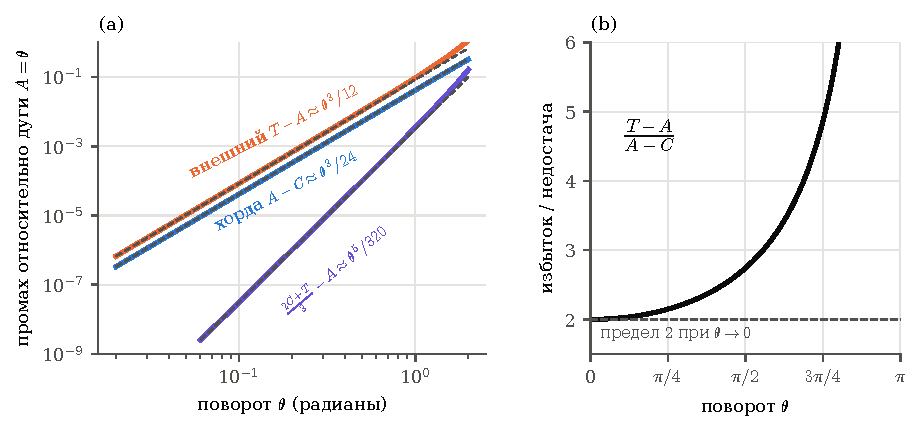
\includegraphics[width=\linewidth]{figures/fig_lengths.pdf}
\caption{Длины. \textbf{(a)} Недостача хорды $A-C$ и избыток внешнего пути
$T-A$ убывают как $\theta^3$, а именно как $\theta^3/24$ и $\theta^3/12$ (штриховые линии: главные члены из
предложения~\ref{prop:lengths}); смесь Снеллиуса~--- Гюйгенса $2{:}1$ убывает как
$\theta^5/320$. \textbf{(b)} Отношение избытка к недостаче равно $2$ в пределе и
растёт с ростом поворота; сокращение~--- утверждение о малых углах.}
\label{fig:lengths}
\end{figure}

\section{Поворот как число}\label{sec:number}

Будем понимать поворот как комплексное число $U=e^{i\theta}$. Тогда хорда~--- это комплексное
число $U-1$, и
\[
U-1=2i\sin(\theta/2)\,e^{i\theta/2}.
\]
Её длина равна $C$, а её направление~--- это начальное направление, повёрнутое на $\theta/2$ (плюс
четверть оборота). \emph{Хорда поворачивается вдвое медленнее отрезка.} Полный оборот
отрезка, $\theta=2\pi$, поворачивает направление хорды лишь на полуоборот.

\paragraph{Хорда и сходство.} Положим
\[
S=\cos^2(\theta/2)=\tfrac12(1+\operatorname{Re}U),\qquad d=\sin(\theta/2)=\tfrac12 C.
\]
Тогда $S+d^2=1$ и $1-S=C^2/4$. Это тождество из статьи о двойном накрытии
\cite{davis-dc}, где $d$ понимается как половина хорды, а $S$~--- как сходство двух
положений. Два положения полностью одинаковы ($S=1$), когда хорда обращается в нуль. Они
полностью различны ($S=0$) при полуобороте, когда хорда~--- диаметр.

\paragraph{Касательная и отображение Кэли.} Отрезок касательной $\tau=\tan(\theta/2)$ строит
поворот алгебраически, без экспоненты:
\[
U=\frac{1+i\tau}{1-i\tau},\qquad
\tau=\frac{\sin\theta}{1+\cos\theta}=\frac{\operatorname{Im}U}{1+\operatorname{Re}U}=
\frac{\operatorname{Im}U}{2S}.
\]
Это преобразование Кэли \cite{cayley}. При $\theta\to\pi$ имеем $\tau\to\infty$: при
полуобороте две касательные параллельны, никогда не пересекаются, и у внешнего пути нет
вершины. Отображение Кэли достигает любого поворота, кроме полуоборота.

\begin{plain}
Как число поворот~--- это точка на единичной окружности. Путь напрямик~--- это «где ты
сейчас минус где ты начинал». Его направление поворачивается вдвое медленнее палки, поэтому
один полный оборот палки поворачивает путь напрямик только на полуоборот. Половина длины
пути напрямик~--- это в точности расстояние $d$ в тождестве двойного накрытия $S+d^2=1$, так
что путь напрямик измеряет, насколько различны два положения. Отрезок обхода~--- то
единственное число, которое восстанавливает весь поворот одной арифметикой, без экспонент.
При полуобороте он ломается: две боковые линии параллельны и никогда не встречаются.
\end{plain}

\section{Энергия}\label{sec:energy}

В решёточной калибровочной теории поворот $U$~--- это голономия по границе грани, а энергия
грани измеряет, насколько $U$ далёк от $1$ \cite{wilson}. Каждый из трёх путей даёт
энергию:
\[
C^2=2(1-\cos\theta)=\theta^2-\tfrac{1}{12}\theta^4+\tfrac{1}{360}\theta^6-\dots,\qquad
A^2=\theta^2,\qquad
T^2=\theta^2+\tfrac16\theta^4+\tfrac{17}{720}\theta^6+\dots
\]
$C^2$~--- это действие Вильсона (с точностью до нормировки), а $A^2$~--- геодезическое
действие Мантона \cite{manton}, то есть континуальная энергия грани. Касательная энергия снова
промахивается с другой стороны, и снова ровно вдвое сильнее в главном порядке. Поэтому те же
веса Снеллиуса~--- Гюйгенса её сокращают.

\begin{proposition}\label{prop:energy}
\[
\frac{2C^2+T^2}{3}=\theta^2+\tfrac{7}{720}\theta^6+\tfrac{1}{1008}\theta^8+O(\theta^{10}).
\]
Член с $\theta^4$ сокращается точно. Эта комбинация алгебраична по $U$:
$C^2=|U-1|^2$ и $T^2=4\,|\operatorname{Im}U|^2/(1+\operatorname{Re}U)^2$.
\end{proposition}

\begin{plain}
Энергию поворота можно измерять по пути напрямик, по истинному пути или по обходу.
Решёточная физика с 1974 года пользуется путём напрямик, потому что его легко вычислять;
истинный путь~--- это то, что имеет в виду континуум. Энергия по пути напрямик чуть меньше,
чем нужно, а энергия по обходу чуть больше, причём вдвое сильнее. Смесь в пропорции два к
одному сокращает главную ошибку, и для этого нужна только арифметика над $U$.
\end{plain}

\begin{figure}[t]\centering
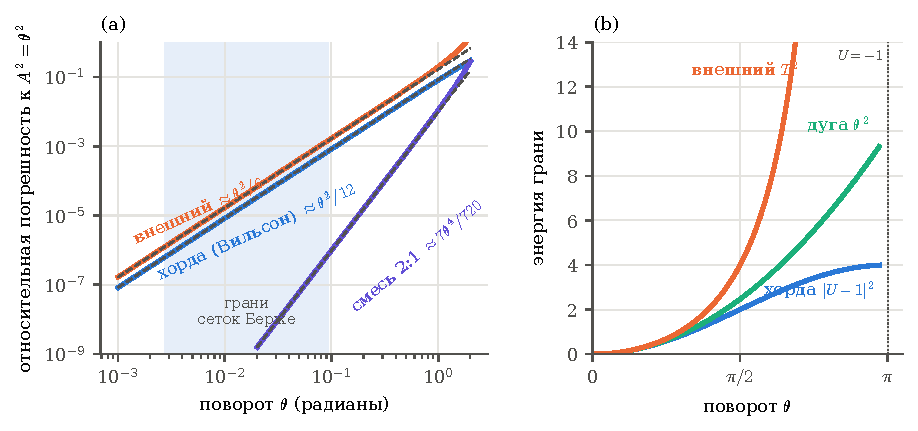
\includegraphics[width=\linewidth]{figures/fig_energy.pdf}
\caption{Энергия. \textbf{(a)} Относительная ошибка каждой энергии грани по сравнению с
континуальной энергией $\theta^2$: у хорды (действие Вильсона) она равна $\theta^2/12$, у внешнего
пути~--- $\theta^2/6$, у смеси $2{:}1$~--- $7\theta^4/720$ (предложение~\ref{prop:energy};
штриховые линии~--- главные члены). Затенённая полоса~--- диапазон углов граней на сетках
$SU(2)$ с метрикой Берже из раздела~\ref{sec:mesh}, от медианы при $n=5$ до наибольшего угла при $n=1$.
\textbf{(b)} Три энергии во всём диапазоне поворотов: энергия хорды ограничена числом $4$,
энергия дуги равна $\theta^2$, а у энергии внешнего пути есть барьер при $U=-1$.}
\label{fig:energy}
\end{figure}

\begin{remark}[Что это исправляет и чего не исправляет]
На решётке с шагом $a$ и для гладкого поля $\theta=O(a^2)$, так что член с $\theta^4$~--- это
относительная поправка порядка $a^4$. Главная решёточная ошибка имеет порядок $a^2$ и
происходит от формы грани, а не от компактности группы; именно её устраняет улучшение
Симанзика \cite{lw}. Приведённая выше комбинация затрагивает только ошибку компактности.
Эта ошибка существенна для сильных полей и грубых решёток и пренебрежимо мала для гладких
полей на мелких решётках. Кроме того, касательная энергия расходится при полуобороте $U=-1$,
в отличие от энергии Вильсона и подобно отображению Кэли. Решёточные действия ровно с таким
барьером изучались как действия, сохраняющие топологию \cite{luscher,fukaya}: они замораживают
топологию в методе Монте-Карло, а Кройц утверждал, что такие условия допустимости несовместимы с
положительностью трансфер-матрицы \cite{creutz}. Как этот барьер ведёт себя в моделировании для
смеси, здесь не исследуется.
\end{remark}

\section{Неабелев поворот}\label{sec:su2}

Единичный кватернион (элемент $SU(2)$) имеет вид $U=\cos a+n\sin a$, где $n$~--- чисто мнимый
единичный кватернион. Всё сказанное выше переносится на этот случай с заменой $\theta$ на
геодезический угол $a$ на $S^3$:
\[
|U-1|=2\sin(a/2),\qquad \log U=a\,n,\qquad
U=(1+v)(1-v)^{-1}\ \text{где}\ v=\frac{\operatorname{Im}U}{1+\operatorname{Re}U},\ |v|=\tan(a/2).
\]
Кватернион $U$ поворачивает трёхмерное пространство на угол $2a$, так что хорда, дуга и внешний
путь кватерниона живут на двойном накрытии описываемого им вращения. Вектор Кэли $v$
снова достигает всего, кроме $U=-1$~--- копии единицы на другом листе накрытия.
Скрипт \texttt{verify.py} проверяет все три формулы на $2{,}000$ случайных кватернионах. Хорда
и дуга совпадают с точностью до $10^{-14}$. Восстановление по Кэли совпадает с точностью до
$10^{-10}$; его число обусловленности растёт как $1/(1+\cos a)$ вблизи полуоборота.

\begin{plain}
Те же три пути существуют и для поворотов в трёх измерениях, записанных кватернионами.
Формулы те же самые, только угол поворота измеряется на трёхмерной сфере. Обход
по-прежнему восстанавливает поворот простой арифметикой и по-прежнему ломается только при
полуобороте.
\end{plain}

У вектора Кэли есть наглядный образ. Поскольку $v=\operatorname{Im}U/(1+\operatorname{Re}U)$,
это стереографическая проекция $U$ из точки $-1$ на экваториальное пространство
$\operatorname{Re}U=0$. Рисунок~\ref{fig:cayley} изображает её на одно измерение ниже, на $S^2$.

\begin{figure}[t]\centering
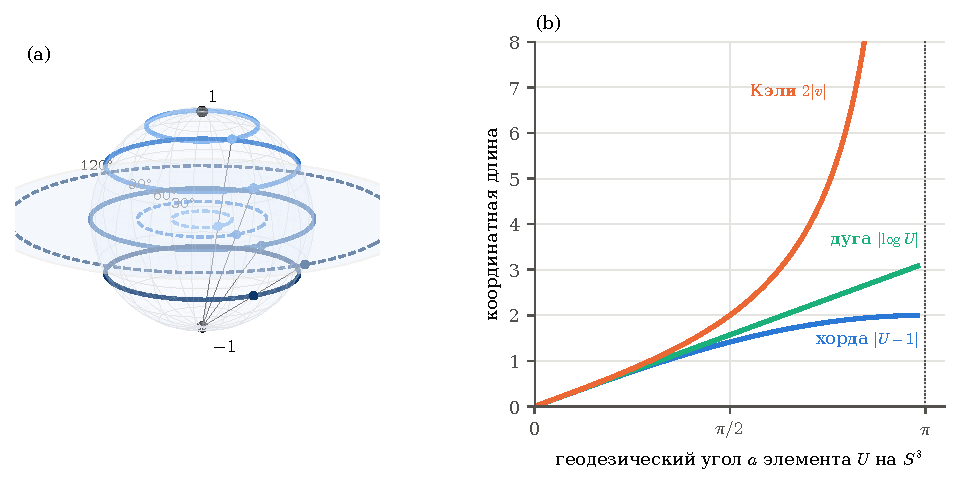
\includegraphics[width=\linewidth]{figures/fig_cayley_3d.pdf}
\caption{Вектор Кэли как стереографическая проекция, изображённая на $S^2$ вместо $S^3$.
\textbf{(a)} Вертикальная ось~--- $\operatorname{Re}U$. Сплошные окружности~--- повороты на
геодезический угол $a=30^\circ,60^\circ,90^\circ,120^\circ$ от $1$; штриховые окружности того же
оттенка~--- их образы Кэли в плоскости $\operatorname{Re}U=0$, радиуса $\tan(a/2)$. Тонкие
лучи исходят из точки проекции $-1$. При $a\to\pi$ образ уходит на бесконечность, поэтому
отображение Кэли достигает всего, кроме $U=-1$. \textbf{(b)} Три координаты одного
поворота: хорда $|U-1|=2\sin(a/2)$, дуга $|\log U|=a$ и координата Кэли $2|v|=2\tan(a/2)$. Это
длины $C$, $A$ и $T$ из раздела~\ref{sec:lengths}, прочитанные на $S^3$.}
\label{fig:cayley}
\end{figure}

\section{Шаги по времени}\label{sec:time}

Возьмём простейшее движение, которое поворачивает: $y'=i\,y$; его точное решение идёт по
окружности. Один шаг $s$ должен повернуть $y$ на $s$. Три классических одношаговых правила
помещают точку в три разных места, и это снова три пути.

\begin{itemize}
  \item \textbf{Явный метод Эйлера}, $y\mapsto(1+is)\,y$, шагает вдоль касательной. Его
    модуль равен $\sqrt{1+s^2}>1$, поэтому он уходит с окружности наружу и на каждом шаге набирает энергию.
  \item \textbf{Неявный метод Эйлера}, $y\mapsto y/(1-is)$, имеет модуль $1/\sqrt{1+s^2}<1$. Он падает
    внутрь окружности и на каждом шаге теряет энергию.
  \item \textbf{Метод Кранка~--- Николсон}, $y\mapsto\frac{1+is/2}{1-is/2}\,y$, есть отображение Кэли с
    $\tau=s/2$. Он остаётся точно на окружности, но поворачивает на $\varphi=2\arctan(s/2)$. Шаг
    $s$ играет роль внешнего пути $T$, а фактически совершённый поворот~--- дуга.
    Фазовое запаздывание равно $s-\varphi=\tfrac{1}{12}s^3+O(s^5)$~--- та же $1/12$, что и в $T-A$ в
    предложении~\ref{prop:lengths}.
\end{itemize}
На рис.~\ref{fig:time} показаны три правила на протяжении одного полного оборота.

\begin{figure}[t]\centering
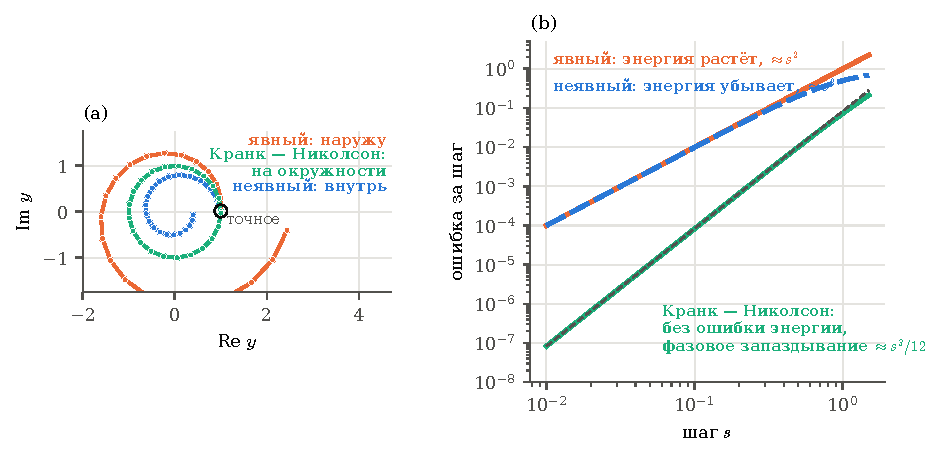
\includegraphics[width=\linewidth]{figures/fig_time.pdf}
\caption{Шаги по времени для $y'=iy$. \textbf{(a)} Двадцать один шаг величины $s=0.3$ (один полный
оборот, $t\approx2\pi$) из $y=1$. Явный метод Эйлера (оранжевый) раскручивается по спирали наружу, неявный метод Эйлера (синий)
закручивается внутрь, а метод Кранка~--- Николсон (зелёный) остаётся на окружности; пустой кружок отмечает точный
конец. \textbf{(b)} Ошибка за шаг: методы Эйлера набирают или теряют энергию порядка $s^2$
(кривые явного и неявного методов совпадают в главном порядке), тогда как метод Кранка~--- Николсон не делает
ошибки в энергии и отстаёт по фазе на $s-2\arctan(s/2)\approx s^3/12$ (штриховая линия).}
\label{fig:time}
\end{figure}

\paragraph{Три спирали, одна из них золотая.} Каждый шаг явного метода Эйлера умножает
модуль на $\sqrt{1+s^2}$ и поворачивает на $\arctan s$, так что отношение роста к повороту никогда
не меняется. Поэтому каждая получаемая им точка лежит точно на логарифмической (равноугольной)
спирали, \emph{spira mirabilis} Якоба Бернулли,
\[
r=e^{b\theta},\qquad b(s)=\frac{\ln(1+s^2)}{2\arctan s}.
\]
Неявный метод Эйлера лежит на зеркальной спирали $r=e^{-b\theta}$, её близнеце с тем же наклоном, а
метод Кранка~--- Николсон~--- член семейства с нулевым наклоном: окружность между ними. При шаге с
рис.~\ref{fig:time}(a), $s=0.3$, внешняя спираль растёт в $1.2614$ раза за каждую четверть
оборота, при наклоне $8.41^\circ$. Золотая спираль~--- это член семейства, растущий в
$\varphi=(1+\sqrt5)/2$ раз за каждую четверть оборота, $b=2\ln\varphi/\pi\approx0.3063$, при наклоне
$17.03^\circ$. Спираль Фибоначчи из четвертей окружностей, вписанных в квадраты, приближает её, потому что
отношения соседних чисел Фибоначчи стремятся к $\varphi$. Поскольку $b(s)$ возрастает по $s$,
существует ровно один шаг, при котором явный метод Эйлера точно вычерчивает золотую спираль:
$s^\ast\approx0.6515$, или $33.08^\circ$ поворота за шаг. Золотой случай принадлежит этому единственному
шагу. Это член семейства, которое рисует метод, а не свойство самого метода.

Для общего линейного потока $y'=-Gy$ множитель Кранка~--- Николсон
$r(z)=(1-z/2)/(1+z/2)$ удовлетворяет $|r(z)|\le1$ ровно тогда, когда $\operatorname{Re}z\ge0$. Его
поведение на ненормальной матрице $G$ определяется числовым образом $W(G)$. По теореме
Крузе~--- Паленсии \cite{cp}, $\|r(hG)^k\|\le(1+\sqrt2)\sup_{z\in W(G)}|r(hz)|^k$. На группе
Ли отображение Кэли сохраняет каждое обновление точно на $SU(2)$ \cite{iserles}.

\begin{plain}
Моделировать что-то вращающееся~--- значит продвигать его вперёд понемногу, шаг за шагом. Самый простой
шаг уходит вдоль боковой линии и сползает наружу, набирая энергию, которой у него быть не должно.
Обратный вариант сползает внутрь и теряет энергию. Шаг Кэли, отрезок обхода, остаётся
точно на окружности и лишь немного отстаёт~--- на ту же одну двенадцатую, что отделяет
обход от истинного пути. Если нарисовать много шагов, сползание наружу вычерчивает логарифмическую
спираль, из того же семейства, что и золотая спираль, а при одном размере шага она в точности золотая.
Сползание внутрь~--- её зеркальный близнец, а шаг Кэли~--- окружность между ними. Поэтому
он оказался естественным правилом для моделирования потока на сетке, и сопутствующая статья теперь им
пользуется: восемь шагов Кэли следуют за потоком так же точно, как много маленьких явных шагов. Собственные
часы движка по-прежнему шагают вдоль истинной кривой (раздел~\ref{sec:gigi}).
\end{plain}

\section{Близнецы, обратная сторона и Бертран}\label{sec:twins}

\paragraph{У каждого промаха есть близнец с другой стороны.} Оценка Снеллиуса~--- Гюйгенса
$(2C+T)/3$ даёт избыток относительно дуги. Другая оценка Снеллиуса даёт недостачу:
\[
L=\frac{6\sin(\theta/2)}{2+\cos(\theta/2)},\qquad
\theta-L=\tfrac{1}{2880}\theta^5+O(\theta^7),\qquad L<\theta<\frac{2C+T}{3}.
\]
Два промаха равны $\theta^5/320$ сверху и $\theta^5/2880$ снизу, девять к одному. Значит, близнецов
можно снова смешать, $\tfrac{1}{10}\bigl(9L+\tfrac{2C+T}{3}\bigr)=\theta+O(\theta^7)$, и
смесь оставляет меньшую пару близнецов. Каждое сокращение порождает следующее.

\paragraph{Близнец с обратной стороны.} Хорда не знает, в какую сторону шёл поворот.
Повороты $\theta$ и $2\pi-\theta$ имеют одну и ту же хорду. Внешний путь знает: его
отрезок касательной меняет знак, $\tan\bigl((2\pi-\theta)/2\bigr)=-\tan(\theta/2)$, потому что
вершина, где встречаются касательные, переходит на другую сторону окружности.

\paragraph{Где находится вершина.} Прямая хорды лежит на расстоянии $p=\cos(\theta/2)$
от центра, а вершина~--- на расстоянии $1/p$ (полюс и поляра). Положение вершины
определяет режим.
\begin{itemize}
  \item \emph{Вершина вне окружности} ($0<p<1$): всё вещественно.
  \item \emph{Прямая хорды проходит через центр} ($p=0$, полуоборот): касательные
    параллельны, и вершина находится в бесконечности. За этой точкой вершина возвращается с обратной стороны;
    это близнец с обратной стороны. Переход через центр переключает на близнеца, и всё остаётся вещественным.
  \item \emph{Вершина внутри окружности} ($p>1$; прямая хорды не пересекает окружность):
    две концевые точки становятся комплексно сопряжённой парой, и поворот становится мнимым,
    $\theta=i\varphi$. Тогда $C=2i\sinh(\varphi/2)$, отрезок касательной равен $i\tanh(\varphi/2)$, и
    $S=\cosh^2(\varphi/2)>1$. Тождество $S+d^2=1$ сохраняется, с мнимым $d=i\sinh(\varphi/2)$.
    Окружность превратилась в гиперболу, а поворот~--- в буст. Именно переход через границу окружности
    делает числа невещественными.
\end{itemize}

\paragraph{Парадокс Бертрана.} Бертран спросил, какова вероятность того, что «случайная хорда»
длиннее стороны вписанного правильного треугольника \cite{bertrand}. Ответ
зависит от того, как выбирается хорда, и каждый классический способ делает равномерно распределённой
одну из величин этой статьи:
\begin{center}\small
\begin{tabular}{lll}\toprule
Способ выбора хорды & Равномерная величина & Вероятность \\ \midrule
две случайные концевые точки & дуга $\theta$ & $1/3$ \\
случайное расстояние вдоль радиуса & $\sqrt S=\cos(\theta/2)$ & $1/2$ \\
случайная середина & сходство $S$ & $1/4$ \\
\bottomrule\end{tabular}
\end{center}
Хорда больше $\sqrt3$ ровно тогда, когда $\theta>2\pi/3$, $\cos(\theta/2)<1/2$ и $S<1/4$, так что
три ответа получаются сразу. Моделирование с двумя миллионами хорд на каждый способ даёт
$0.3333$, $0.5004$ и $0.2498$. Внешний путь не даёт четвёртого ответа такого рода: его отрезок уходит в
бесконечность при полуобороте, поэтому его нельзя распределить равномерно. Джейнс утверждал, что инвариантность
относительно сдвигов и изменения масштаба окружности выделяет способ с радиусом \cite{jaynes}.

Группа поворотов всё же даёт четвёртый ответ, потому что у неё есть собственный честный способ
выбрать поворот случайно~--- мера Хаара, которая не оставляет нам никакого выбора. Для равномерно
распределённого случайного единичного кватерниона геодезический угол $a$ имеет плотность $(2/\pi)\sin^2a$ на $[0,\pi]$, поэтому
сходство $S=\cos^2(a/2)$ подчиняется закону полукруга $(8/\pi)\sqrt{S(1-S)}$ на $[0,1]$. Событие
Бертрана~--- это $S<1/4$, и его вероятность равна
\[
\tfrac13-\tfrac{\sqrt3}{4\pi}\approx0.19550,
\]
что не совпадает ни с одним из трёх классических ответов. Моделирование четырёх миллионов случайных поворотов даёт
$0.19545$ (\path{scripts/haar_sameness.py} в репозитории GIGI).

\begin{plain}
У каждой оценки, которая промахивается в одну сторону, есть близнец, промахивающийся в другую, и смешивание
близнецов убирает промах, оставляя пару поменьше. У хорды тоже есть поворот-близнец: если пойти длинным
путём вокруг, хорда будет та же, но обход это замечает, потому что его вершина перескакивает на
другую сторону. Где стоит эта вершина, решает всё. Снаружи окружности всё вещественно.
Через центр~--- вы переходите к близнецу. Внутри окружности числа становятся мнимыми,
окружность становится гиперболой, и всё равно $S+d^2=1$ выполняется. Знаменитый парадокс Бертрана~--- это
тот же вопрос в другом обличье: «случайная хорда» ничего не значит, пока вы не скажете, какую из этих
величин вы распределяете равномерно: дугу, квадратный корень из сходства или само
сходство.
\end{plain}

\section{Игра в билеты}\label{sec:tickets}

Каждый из предыдущих разделов рассматривает одну сторону поворота. Этот раздел собирает их
в одной комнате. Всё в нём элементарно, и каждое число проверено скриптом \texttt{verify.py}.
Смысл не в новой математике, а в том, что три пути, энергия, близнецы и треугольник
Бертрана появляются, стоит только задать простой вопрос о ходьбе.

\paragraph{Правила.} Все начинают в центре $O$ комнаты. Каждому выдают
билеты, и билет оплачивает один ход по прямой длины не более $1$. Два игрока, $A$ и
$B$, тратят по одному билету, уходя из $O$ каждый в выбранном им направлении, так что
они оказываются на единичной окружности под углом $\theta$ друг к другу. Теперь $A$ хочет снова встретиться с $B$. Одно
правило не ослабляется никогда: ни один ход не может стоить больше одного билета.

\paragraph{Три цены одного перехода.} У перехода есть три естественные цены, по одной
на каждый способ его измерить.
\begin{itemize}
  \item \emph{Дуга}, путь, которым шёл поворот, стоит $\theta$ билетов. Она укладывается в один билет
    вплоть до ровно одного радиана, $57.30^\circ$. Это и есть радиан: угол, дуга которого
    имеет длину в один билет.
  \item \emph{Хорда}, напрямик, стоит $2\sin(\theta/2)$. Она укладывается в один билет вплоть
    до ровно $60^\circ$. Тогда $A$, $B$ и $O$ образуют равносторонний треугольник, а шесть
    игроков, расставленных через $60^\circ$, стоят в вершинах правильного шестиугольника, стороны которого
    равны его радиусу. С этого шестиугольника начинал Архимед.
  \item \emph{Энергия} в решёточном счёте "--- это энергия грани Вильсона
    $1-\cos\theta=\tfrac12C^2$. В этих единицах один ход длины $L$ стоит
    $\tfrac12L^2$, так что два хода по радиусам обратно через центр вместе стоят
    $\tfrac12+\tfrac12=1$. Назовём это одним билетом энергии. Переход стоит
    ровно один билет энергии при $90^\circ$, меньше при меньших углах и больше при больших, вплоть до двух на
    противоположной стороне комнаты.
\end{itemize}
У каждой цены свой угол в один билет, и все три различны.
\begin{center}\small
\begin{tabular}{llll}\toprule
Цена & Стоимость перехода & Один билет при & Почему \\ \midrule
дуга & $\theta$ & $57.30^\circ$ & определение радиана \\
хорда & $2\sin(\theta/2)$ & $60^\circ$ & равносторонний треугольник \\
энергия & $1-\cos\theta$ & $90^\circ$ & Пифагор \\
\bottomrule\end{tabular}
\end{center}

\paragraph{Вся доска.} Таблица выше оценивает переход тремя способами, но у каждого
пути есть и длина, и энергия, так что на доске шесть клеток, и каждая однозначно определена,
как только зафиксировано её правило. Если энергию измерять как $\tfrac12L^2$, как выше:
\begin{center}\small
\begin{tabular}{lccc}\toprule
Один билет\ldots & внешний путь & дуга & хорда \\ \midrule
длины & $53.13^\circ$ & $57.30^\circ$ & $60^\circ$ \\
 & треугольник $3$--$4$--$5$ & один радиан & шестиугольник \\[2pt]
энергии & $70.53^\circ$ & $81.03^\circ$ & $90^\circ$ \\
 & $\cos\theta=\tfrac13$ & $\sqrt2$ радиан & квадрат \\
\bottomrule\end{tabular}
\end{center}
В каждой строке внешний путь, самый дорогой, покупает наименьший поворот, а хорда, самая
дешёвая, "--- наибольший. Две клетки сами по себе являются классическими углами.
Внешний путь покупает один билет длины, когда его отрезок касательной $\tan(\theta/2)=\tfrac12$, и
построение Кэли с таким отрезком даёт точку $(\tfrac35,\tfrac45)$. При любом рациональном
отрезке $t$ построение даёт рациональную точку $\bigl((1-t^2)/(1+t^2),\,2t/(1+t^2)\bigr)$,
и именно так возникает каждая пифагорова тройка. Внешний путь покупает один билет энергии при
$\cos\theta=\tfrac13$ "--- это двугранный угол правильного тетраэдра.

\paragraph{Зазор.} Между $57.30^\circ$ и $60^\circ$ короткий путь напрямик укладывается в один
билет, а истинный путь "--- нет. Величина этого зазора при угле шестиугольника равна
$\pi/3-1\approx0.0472$ билета, надбавка в $4.72\%$, и это то же число, что
отношение длины окружности к периметру шестиугольника, $2\pi/6$, минус один. Это
цена кривизны в масштабе одного билета. Именно это вычисляется в разделе~\ref{sec:lengths},
$A-C\approx\theta^3/24$, только увиденное в размере, который можно пройти ногами.

\paragraph{Почему энергия окупается именно при $90^\circ$.} Квадрат перехода равен
$|A-B|^2=|A|^2+|B|^2-2A\cdot B=2-2\cos\theta$. Путь обратно через центр состоит из двух
отрезков длины один. По энергии переход и два отрезка стоят одинаково ровно тогда, когда
$A\cdot B=0$: при прямом угле, где хорда "--- гипотенуза двух билетов.
Ниже $90^\circ$ срезать напрямик выгодно по энергии. Выше $90^\circ$ два отдельных хода
через центр обходятся по энергии дешевле, чем один переход. Энергия растёт как
квадрат длины, поэтому разбиение длинного хода на два коротких экономит энергию, и за
прямым углом разбиение выигрывает.

\paragraph{Целые билеты: почему всегда два хода.} Теперь ужесточим правило: билет
нужно тратить целиком, так что каждый ход имеет длину ровно один. С одним целым билетом $A$
может попасть только на окружность радиуса один вокруг $A$. Если $B$ не стоит точно там
(при $\theta=60^\circ$), $A$ перелетает или недотягивает. С двумя целыми билетами $A$ может
достичь любой точки на расстоянии не больше двух, но вершина, в которой $A$ поворачивает, должна лежать в одном билете
от $A$ и в одном билете от $B$. Две окружности радиуса один вокруг $A$ и $B$ пересекаются ровно
в двух точках, симметричных относительно хорды. Одна из них "--- центр $O$; другая "--- его
отражение относительно середины хорды, точка $A+B$. Итак, существует ровно два
маршрута из двух билетов:
\begin{itemize}
  \item \emph{через центр}: дойти домой, затем выйти по пути $B$;
  \item \emph{через вершину-близнеца} $A+B$, вершину, противоположную $O$ в ромбе
    $O$, $A$, $A+B$, $B$, все четыре стороны которого имеют длину один.
\end{itemize}
Эти две вершины "--- близнецы в смысле раздела~\ref{sec:twins}: два ответа на один
вопрос, зеркальные отражения друг друга относительно хорды. При полуобороте они сливаются, поскольку $A+B=O$
при $B=-A$, и остаётся только маршрут через центр.

\paragraph{Где стоит вершина-близнец.} Вершина-близнец находится на расстоянии
$|A+B|=2\cos(\theta/2)$ от центра, вдвое дальше середины хорды. Она
лежит вне круга при углах меньше $120^\circ$, внутри при больших и ровно на окружности при
$120^\circ$. При этом угле переход равен $\sqrt3$, стороне треугольника Бертрана, и
вершина-близнец попадает в вершину шестиугольника между двумя игроками: ромб распадается
на два равносторонних треугольника.

\paragraph{Где стоит вершина обхода.} Внешний путь из раздела~\ref{sec:picture}
поворачивает в вершине касательных $Q$, на расстоянии $\sec(\theta/2)$ от центра на той же
биссектрисе. Вершина касательных и вершина-близнец совпадают ровно тогда, когда
$\sec(\theta/2)=2\cos(\theta/2)$, то есть при $\theta=90^\circ$. Тогда ромб "--- это
квадрат, его дальняя вершина "--- точка пересечения касательных, каждый отрезок касательной равен $\tan45^\circ=1$,
и внешний путь составляет ровно два целых билета. Ниже $90^\circ$ вершина касательных "---
ближняя из двух, и обход стоит меньше двух билетов; выше $90^\circ$ она
дальняя, и обход стоит больше.

\paragraph{Близнец прямого угла.} Энергия перехода к $B$ равна $1-\cos\theta$;
энергия перехода к точке, противоположной $B$, равна $1+\cos\theta$. В сумме они всегда дают два
билета, потому что $A$, $B$ и $-B$ образуют прямой угол при $A$ (Фалес). В обозначениях
раздела~\ref{sec:number} эти две энергии равны в точности $2d^2$ и $2S$, так что это снова $S+d^2=1$,
а точка безубыточности при $90^\circ$ "--- это точка, где $S=d^2=\tfrac12$: два
положения ровно настолько же одинаковы, насколько различны.

\paragraph{Какое правило энергии.} Прямой угол "--- точка безубыточности для правила Вильсона, энергия
$\tfrac12C^2$. Это правило, а не факт о комнате. С правилом континуума, энергия
$\tfrac12\theta^2$, точка безубыточности сдвигается к $81.03^\circ$; с правилом внешнего пути,
$\tfrac12T^2$, "--- к $70.53^\circ$. Выбор между ними определяется пределом малых билетов, где
правила обязаны согласовываться с континуумом: при $5^\circ$ три энергии равны $0.003805$,
$0.003808$ и $0.003813$, в пределах $0.2\%$, и они становятся одинаковыми по мере того, как билеты уменьшаются.
Именно на больших поворотах решёточные правила расходятся, и раздел~\ref{sec:energy} посвящён как раз
этому различию.

Итак, прямой угол особенный трижды. По правилу Вильсона переход стоит один
билет энергии, и его энергия равна энергии двух ходов через центр. Вообще без всякого правила,
из одной лишь геометрии, обход становится двумя целыми билетами, через вершину квадрата.

\begin{table}[h!]\centering\small
\caption{Игра в билеты при пяти углах: три цены перехода, его энергия
Вильсона и расстояния от центра до вершины-близнеца $A+B$ и до вершины
касательных $Q$.}
\label{tab:tickets}
\begin{tabular}{rrrrrrr}\toprule
$\theta$ & дуга & хорда & внешний путь & энергия & вершина-близнец & вершина касательных \\ \midrule
$57.30^\circ$ & 1.0000 & 0.9589 & 1.0926 & 0.4597 & 1.7552 & 1.1395 \\
$60^\circ$ & 1.0472 & 1.0000 & 1.1547 & 0.5000 & 1.7321 & 1.1547 \\
$90^\circ$ & 1.5708 & 1.4142 & 2.0000 & 1.0000 & 1.4142 & 1.4142 \\
$120^\circ$ & 2.0944 & 1.7321 & 3.4641 & 1.5000 & 1.0000 & 2.0000 \\
$180^\circ$ & 3.1416 & 2.0000 & $\infty$ & 2.0000 & 0 & $\infty$ \\
\bottomrule\end{tabular}
\end{table}

\begin{figure}[h!]\centering
\begin{tikzpicture}[scale=2.6]
  \def\t{70}
  \coordinate (O) at (0,0);
  \coordinate (A) at (1,0);
  \coordinate (B) at ({cos(\t)},{sin(\t)});
  \coordinate (P) at ({1+cos(\t)},{sin(\t)});
  \coordinate (Q) at (1,{tan(\t/2)});
  \draw[gray!50] (O) circle (1);
  \draw[thick] (O) -- (A); \draw[thick] (O) -- (B);
  \draw[gray,dotted,thick] (A) -- (P) -- (B);
  \draw[very thick,dgarc] (A) arc (0:\t:1);
  \draw[very thick,dgchord] (A) -- (B);
  \draw[very thick,dgtan] (A) -- (Q) -- (B);
  \fill (O) circle (0.022) node[below left] {$O$};
  \fill (A) circle (0.022) node[below right] {$A$};
  \fill (B) circle (0.022) node[above left] {$B$};
  \fill[gray] (P) circle (0.022) node[above right] {$A+B$};
  \fill[dgtan] (Q) circle (0.022) node[right] {$Q$};
  \draw (0.2,0) arc (0:\t:0.2); \node at ({0.29*cos(\t/2)},{0.29*sin(\t/2)}) {$\theta$};
\end{tikzpicture}
\caption{Игра в билеты при $\theta=70^\circ$. Каждый игрок прошёл от
центра на один билет. Хорда (синяя), дуга (зелёная) и внешний путь через вершину касательных $Q$
(оранжевый) "--- три цены перехода. Два маршрута из целых билетов поворачивают в
центре или в его близнеце $A+B$, дальней вершине единичного ромба (пунктир). При $90^\circ$
вершина касательных и вершина-близнец совпадают.}
\label{fig:tickets}
\end{figure}

\begin{plain}
Представьте комнату. Все начинают в середине с билетами, и один билет оплачивает один
проход по прямой не длиннее одного шага. Двое друзей тратят по билету и расходятся в
разные стороны. Как одному вернуться к другому? Пройти по кривой стоит один
билет, только если между ними не больше примерно $57^\circ$. Срезать напрямик стоит один
билет, если между ними не больше $60^\circ$. Если считать так, как физики считают энергию,
прямой переход стоит один билет ровно при $90^\circ$ "--- столько же, сколько вернуться в
середину и снова выйти; это Пифагор. Если билеты нужно тратить целиком, всегда есть
ровно два способа сделать это за два хода: повернуть в середине комнаты или повернуть в
её зеркальном углу по другую сторону перехода. Эти два угла "--- близнецы. При
$120^\circ$ угол-близнец попадает прямо на окружность, а при $90^\circ$ он становится
вершиной идеального квадрата, где встречаются две боковые линии и внешний путь равен ровно
двум целым билетам.
\end{plain}

\section{Насколько это важно на реальной сетке}\label{sec:mesh}

Наша работа по восстановлению кривизны~\cite{davis-rtc} измеряет $SU(2)$-силу на сетках гомологической
сферы Пуанкаре при связности Леви-Чивиты метрики Берже. Её нативное действие~--- энергия
хорды: дефект каждой грани равен $D=U_f-1$. В таблице~\ref{tab:angles} приведены углы граней $a$
на этих сетках (\texttt{face\_angles.py}, по зафиксированным входным данным), а
на рис.~\ref{fig:faces} показаны их распределения.

\begin{table}[h!]\centering\small
\caption{Углы голономии граней на сетках $SU(2)$ с метрикой Берже и относительный разрыв между
энергией хорды и энергией дуги при наибольшем угле, $a^2/12$.}
\label{tab:angles}
\begin{tabular}{rrrrr}\toprule
$n$ & число граней & медиана $a$ & макс. $a$ & разрыв энергий хорды и дуги при макс. \\ \midrule
1 & 480 & 0.0684 & 0.0937 & $7.3\times10^{-4}$ \\
2 & 3{,}840 & 0.0172 & 0.0250 & $5.2\times10^{-5}$ \\
3 & 12{,}960 & 0.0076 & 0.0113 & $1.1\times10^{-5}$ \\
5 & 60{,}000 & 0.0027 & 0.0041 & $1.4\times10^{-6}$ \\
\bottomrule\end{tabular}
\end{table}

\begin{figure}[t]\centering
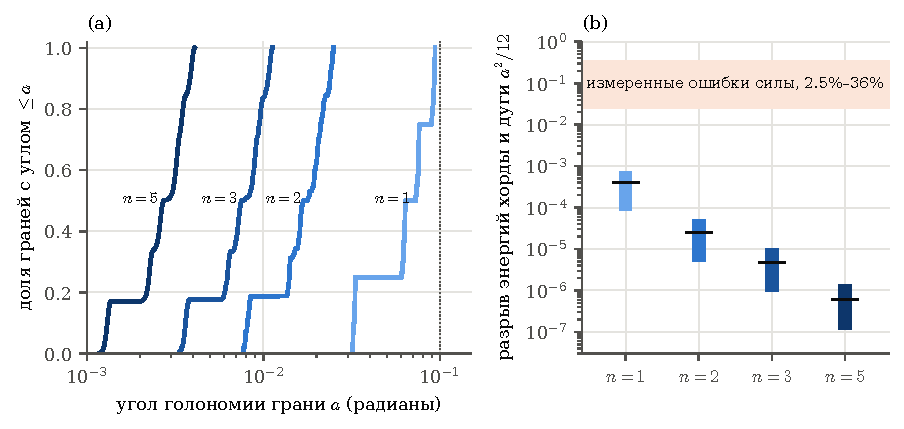
\includegraphics[width=\linewidth]{figures/fig_face_angles.pdf}
\caption{Углы граней на сетках $SU(2)$ с метрикой Берже по зафиксированным входным данным (числа
таблицы~\ref{tab:angles}; \texttt{make\_figures.py} проверяет, что они совпадают). \textbf{(a)}
Функция распределения углов голономии граней на каждом уровне; каждая грань поворачивается менее
чем на $0.1$ радиана. \textbf{(b)} Разрыв энергий хорды и дуги $a^2/12$ по граням: отрезок тянется
от наименьшей грани до наибольшей, а засечка отмечает медиану. Затенённая полоса~--- диапазон
ошибок силы, измеренных на тех же сетках. Разрыв лежит ниже неё на два--пять
порядков.}
\label{fig:faces}
\end{figure}

Углы убывают примерно как площадь грани, а разрыв энергий хорды и дуги всюду меньше
$0.08\%$. Измеренные там ошибки силы составляют от $2.5\%$ до $36\%$. Поэтому
выбор между хордой и дугой не является тем, что ограничивает эту работу, и два используемых там
прочтения (дуга, через $\log U$, для ковариантного восстановления; хорда, $U-1$, для силы)
согласуются с запасом в пределах измеренной ошибки. Где три пути действительно важны для этой
программы, так это во времени: на её самом мелком уровне поток продвигается шагами по правилу Кэли из
раздела~\ref{sec:time}.

\begin{plain}
На сетках, которыми мы на самом деле пользуемся, каждая грань поворачивается меньше чем на десятую
долю радиана. Там короткий путь напрямик и истинный путь различаются по энергии меньше чем на
десятую долю процента, что гораздо меньше ошибок, которые мы измеряем. Так что эта идея не
объясняет те ошибки, и мы говорим об этом прямо. Где она действительно важна, так это в том, как
продвигать движение во времени шаг за шагом, и теперь в той работе для этого используется шаг Кэли.
\end{plain}

\section{Вычисление в GIGI}\label{sec:gigi}

Числа этой статьи находятся в двух местах, и важно, что где. Некоторые из
трёх путей уже входят в GIGI~--- геометрический движок с открытым исходным кодом, в котором
работает наше восстановление кривизны (PolyForm Noncommercial 1.0.0,
\url{https://github.com/nurdymuny/gigi}). Другие пока существуют только в проверочном
скрипте этой статьи. Таблица~\ref{tab:gigi} показывает, что где. Пути указаны относительно корня
репозитория на коммите \texttt{442c13d} ветки \texttt{feat/reading-the-curve}.

\begin{table}[h!]\centering\small
\caption{Где находится каждая идея статьи. «Движок» означает нативный Rust в GIGI;
«скрипт» означает Python в этом каталоге или в \texttt{scripts/} репозитория.}
\label{tab:gigi}
\begin{tabular}{>{\raggedright\arraybackslash}p{4.3cm}>{\raggedright\arraybackslash}p{6.7cm}>{\raggedright\arraybackslash}p{2.2cm}}\toprule
Идея & Где & Вид \\ \midrule
Поворот как число, $q_0=\cos a=\tfrac12\operatorname{Re}\operatorname{tr}U$ &
  примитив \texttt{PLAQUETTE}, \path{src/gauge/plaquette.rs}, одно $q_0$ на грань & движок \\
Половина хорды и сходство, $1-S=d^2=(1-\cos\theta)/2$ &
  \texttt{chord\_d\_sq}, \path{src/dials.rs} & движок \\
Энергия хорды, $D=U_f-1$, взвешенная массой грани &
  \texttt{cell\_action}, \path{src/gauge/ricci_simplicial.rs} & движок \\
Точные связи (перенос вдоль дуги) в метрике Берже &
  \texttt{levi\_civita\_link}, \path{src/gauge/ricci_link.rs} & движок \\
Дуга как отображение, $\exp$ на $\mathfrak{su}(2)$ &
  экспонента Родрига, \path{src/gauge/lie_exp.rs} & движок \\
Шаги по времени &
  \texttt{SYMPLECTIC\_FLOW}: схема чехарды вида «толчок~--- дрейф~--- толчок», дрейф в которой задаётся этой экспонентой,
  \path{src/gauge/symplectic_flow.rs} & движок \\
Углы граней из таблицы~\ref{tab:angles} &
  \texttt{face\_angles.py}, по выходным данным \path{examples/ricci_operator_probe.rs} &
  скрипт на выходе движка \\
Энергия дуги (Мантона), энергия касательной, смесь $2{:}1$ &
  \texttt{verify.py} & скрипт \\
Отображение Кэли и шаг Кранка~--- Николсон & \texttt{verify.py}; на сетке~--- \path{scripts/ricci_su2_pg_flow_cayley.py} & скрипт \\
Сходство по Хаару и Бертран & \path{scripts/haar_sameness.py}, \texttt{verify.py} & скрипт \\
\bottomrule\end{tabular}
\end{table}

\paragraph{Хорда, как её вычисляет движок.} Исходное $SU(2)$-действие из
раздела~\ref{sec:mesh}~--- это в точности энергия хорды. Голономия каждой грани составляется из её
трёх связей, и из её скалярной части вычитается единица:
\begin{lstlisting}[style=rust]
let (a, b, c) = [(0, 3, 1), (0, 4, 2), (1, 5, 2), (3, 5, 4)][face];
let mut h = product(product(u[a], u[b]), inverse(u[c]));
h[0] = h[0] - Jet::constant(1.);      // the chord: D = U_f - 1
...
energy = energy + Jet::constant(2. * mass[(i, j)]) * defects[i][k] * defects[j][k];
\end{lstlisting}
Переменные~--- джеты прямого режима, поэтому тот же проход точно возвращает все восемнадцать
правотривиализованных производных. Углы граней из таблицы~\ref{tab:angles} считаны с того, что этот
код выдал на зафиксированных сетках: нативный зонд \path{examples/ricci_operator_probe.rs},
собранный из приведённого выше исходного кода, исполняемый файл которого закреплён в квитанциях той работы его
SHA-256 (\texttt{71fb30db\ldots}).

\paragraph{Движок шагает вдоль дуги, а не по касательной.} Интегратор GIGI,
\texttt{SYMPLECTIC\_FLOW}, сдвигает каждую связь экспоненциальным отображением, то есть по дуге,
схемой чехарды вида «толчок~--- дрейф~--- толчок», управляемой силой Вильсона. Исследовательский поток
работы по восстановлению кривизны~\cite{davis-rtc} использует метод Рунге~--- Кутты~--- Мунте-Кааса
четвёртого порядка, также построенный на экспоненте, а на самом мелком уровне~--- шаг Кэли из
раздела~\ref{sec:time} (\path{scripts/ricci_su2_pg_flow_cayley.py}). Там шаг был
проверен перед использованием: его отклонение от экспоненты убывает как $|v|^3/12$, его порядок по
времени равен $1.99$, и восемь шагов воспроизводят прогоны четвёртого порядка с точностью до $1.5\%$,
затрачивая от пятой до третьей части вычислений силы. Это исследовательский скрипт. В самом движке
шаг Кранка~--- Николсон пока остаётся предложением, а не описанием.

\paragraph{Чего нет в движке.} Энергия дуги (Мантона), энергия касательной и
комбинация из предложения~\ref{prop:energy} вычисляются только в \texttt{verify.py}. Ни одна из них
не является глаголом движка, и ни одна не проверялась внутри моделирования. Шаг Кэли проверялся, в
описанном выше исследовательском потоке, но и он не является глаголом движка.

\begin{plain}
Часть этой статьи уже есть внутри движка, которым мы пользуемся: он считывает, насколько повернулась
каждая грань, измеряет короткий путь напрямик и строит свою энергию из него, в точности как
предполагает раздел~\ref{sec:mesh}. Его часы двигают всё вдоль истинной кривой. Обход и
смесь два к одному пока живут только в проверочном скрипте. Встроить шаг обхода в
часы движка~--- один из открытых пунктов ниже.
\end{plain}

\section{Чего стоит поворот: к теории Янга~--- Миллса}\label{sec:ym}

\paragraph{Ноль~--- не малая единица; это отсутствие системы.} Одна единица чего угодно реального,
у которой нет ничего, что заставляло бы её предпочесть какое-то направление, простирается одинаково во всех направлениях и ни
по какой оси не может занимать отрицательного пространства. Значит, это сфера, а сфера искривлена. Кривизна
не добавляется к наименьшему объекту; она приходит вместе с самим существованием. В размерности один эта единичная
сфера~--- две точки $-1$ и $+1$. В размерности четыре это трёхмерная сфера единичных
кватернионов, то есть сама калибровочная группа $SU(2)$~--- группа, из которой сделано поле Янга~--- Миллса.
Её кривизна~--- это в точности то, насколько её повороты не коммутируют: при биинвариантной
метрике секционная кривизна плоскости, натянутой на $X$ и $Y$, равна $\tfrac14|[X,Y]|^2$
\cite{milnor}, что на единичных кватернионах равно $1$. Окружность поворотов фотона,
$U(1)$, коммутативна, и она плоская. Центр $SU(2)$, то есть повороты, коммутирующие со всеми
остальными, снова есть в точности $\{-1,+1\}$, а $-1$~--- это полуоборот из раздела~\ref{sec:number},
на котором внешний путь ломается.

\paragraph{Угол создаёт энергию.} Петля поля, которая не повернулась, не несёт
энергии. Петля, повернувшаяся на угол $\theta$, несёт энергию своей хорды,
$1-\cos\theta$ в единицах Вильсона (раздел~\ref{sec:energy}). Два конца не могут встретиться вдоль
дуги бесплатно, потому что дуга принадлежит самому повороту. Любой другой путь через поворот
чего-то стоит: хорда меньше, обход больше.

\paragraph{Энергия приходит целыми билетами.} В игре в билеты из раздела~\ref{sec:tickets}
между отсутствием поворота и одним билетом тратить нечего. Любой переход, который не укладывается в
один билет, требует двух целых проходов с поворотом в центре или в его близнеце.

\paragraph{Вместе.} Наименьшее существующее уже искривлено, а наименьший
обмен~--- целый билет. Между ничем и одной единицей нет ничего. Эта форма~--- пол под энергией
всего существующего~--- и есть то, чем является щель масс. Наша картина говорит,
откуда бы такой пол взялся: из кривизны, которой калибровочная группа обладает просто потому, что она
группа поворотов, а не из кривизны пространства, которая сглаживается по мере роста пространства. По этой же
причине собственное значение $4$, измеренное в сопутствующей статье, не является щелью масс: оно происходит из
кривизны пространства, гомологической сферы Пуанкаре, а не из поля.

\paragraph{Статус.} Изложенная выше геометрия точна и проверена. То, что этот пол \emph{является}
щелью масс Янга~--- Миллса в плоском бесконечном пространстве,~--- это открытая проблема Института Клэя \cite{jaffewitten}, и
эта статья этого не утверждает. Родственные идеи о том, что кривизна в пространстве полей удерживает
энергию выше нуля, восходят к Фейнману \cite{feynman} и Зингеру \cite{singer}. Сопутствующая
заметка в репозитории GIGI (\path{docs/research/unit-curvature-2026-11-18.md})
подробнее разбирает точные части, вместе с родственной литературой.

\begin{plain}
Ноль~--- это не крошечное что-то; это вообще ничто. У наименьшей реальной вещи нет причины
предпочитать одно направление, поэтому она расходится одинаково во все стороны, и это делает её круглой,
а круглое значит искривлённое. Она искривлена просто потому, что существует. Для слабого и сильного ядерных взаимодействий сами
повороты образуют такое круглое, искривлённое пространство ($SU(2)$ и $SU(3)$), и его кривизна~--- это
то, насколько повороты отказываются коммутировать; для света повороты коммутируют, и пространство плоское. Энергии стоит именно поворот, и решётка платит за него по прямому
короткому пути напрямик. В игре в билеты энергия приходит целиком: между нулём билетов и одним
ничего нет. Если сложить всё вместе, это наводит на мысль, что под энергией всего существующего есть пол, а это
то, что физики называют щелью масс. Есть ли такой пол на самом деле у этих сил~--- одна из
великих открытых проблем, и эта статья не утверждает, что решила её.
\end{plain}

\section{Что утверждается и что остаётся открытым}\label{sec:claims}

\textbf{Утверждается}, причём каждый пункт проверен \texttt{verify.py} (все проверки проходят; их число~--- в \texttt{verify\_output.txt}):
\begin{itemize}
  \item порядок длин, промахи $1/24$ и $1/12$ и остаток оценки Снеллиуса~--- Гюйгенса $\theta^5/320$;
  \item направление хорды под половинным углом и $S+d^2=1$, где $d$~--- половина хорды;
  \item построение Кэли в $\mathbb{C}$ и в кватернионах;
  \item ряды для энергии и сокращение $\theta^4$ в $(2C^2+T^2)/3$;
  \item расположение трёх одношаговых правил относительно окружности и фазовое запаздывание Кранка~--- Николсон $s^3/12$;
  \item промах нижнего близнеца $\theta^5/2880$ и смесь $9{:}1$, смена знака на обратной стороне,
    продолжение через границу окружности с сохранением $S+d^2=1$ и три ответа Бертрана;
  \item игра в билеты: углы одного билета ($1$ радиан, $60^\circ$, $90^\circ$),
    точка безубыточности энергии при прямом угле, две вершины для целых билетов $O$ и $A+B$,
    вершина-близнец на окружности при $120^\circ$ и совпадение вершины касательных с вершиной-близнецом при $90^\circ$;
  \item таблица из шести клеток с углами одного билета, близнец Фалеса $2d^2+2S=2$, согласие
    трёх правил энергии при малых поворотах и ответ Хаара $\tfrac13-\sqrt3/(4\pi)$ на вопрос Бертрана;
  \item три спирали шагов по времени: явный и неявный методы Эйлера на зеркальных логарифмических спиралях
    с углом наклона $\arctan b(s)$, метод Кранка~--- Николсон на окружности и единственный золотой шаг $s^\ast\approx0.6515$.
\end{itemize}
Углы граней из таблицы~\ref{tab:angles} измерены по зафиксированным данным.

\textbf{Не утверждается.} Мы не претендуем на приоритет ни в одном из перечисленных выше классических тождеств. Мы не утверждаем, что
комбинированная энергия является лучшим решёточным действием; для этого потребовались бы моделирования и
учёт барьера полуоборота. Мы не утверждаем, что это объясняет какую-либо ошибку в
работе по восстановлению кривизны; раздел~\ref{sec:mesh} показывает, что не объясняет.

\textbf{Открыто.}
\begin{itemize}
  \item Поиск предшествующих работ, содержащих комбинацию энергий из предложения~\ref{prop:energy}, и
    вообще решёточных действий на основе касательной.
  \item Шаг Кэли (Кранка~--- Николсон) внутри движка. Он был проверен в исследовательском
    потоке сопутствующей статьи~\cite{davis-rtc}; собственный интегратор GIGI шагает
    экспонентой (раздел~\ref{sec:gigi}).
  \item Проверка в сильном поле или на грубой решётке, где $\theta$ не мало,~--- единственный режим,
    в котором комбинация энергий могла бы иметь значение.
\end{itemize}

\paragraph{Воспроизводимость.} \texttt{verify.py} и \texttt{face\_angles.py} в этом
каталоге; вывод первого сохранён как \texttt{verify\_output.txt}, второго~--- как
\texttt{face\_angles.json}.

\begin{thebibliography}{99}\small
\bibitem{archimedes} Archimedes, \emph{Measurement of a Circle}, in T.~L.~Heath (ed.), \emph{The Works of Archimedes}, Cambridge University Press, 1897.
\bibitem{snellius} W.~Snellius, \emph{Cyclometricus}, Leiden, 1621.
\bibitem{huygens} C.~Huygens, \emph{De circuli magnitudine inventa}, Leiden, 1654.
\bibitem{cayley} A.~Cayley, Sur quelques propri\'et\'es des d\'eterminants gauches, \emph{J.\ reine angew.\ Math.} 32 (1846) 119--123.
\bibitem{cn} J.~Crank, P.~Nicolson, A practical method for numerical evaluation of solutions of partial differential equations of the heat-conduction type, \emph{Proc.\ Cambridge Philos.\ Soc.} 43 (1947) 50--67.
\bibitem{wilson} K.~G.~Wilson, Confinement of quarks, \emph{Phys.\ Rev.\ D} 10 (1974) 2445--2459.
\bibitem{manton} N.~S.~Manton, An alternative action for lattice gauge theories, \emph{Phys.\ Lett.\ B} 96 (1980) 328--330.
\bibitem{lw} M.~L\"uscher, P.~Weisz, On-shell improved lattice gauge theories, \emph{Commun.\ Math.\ Phys.} 97 (1985) 59--77.
\bibitem{iserles} A.~Iserles, H.~Z.~Munthe-Kaas, S.~P.~N{\o}rsett, A.~Zanna, Lie-group methods, \emph{Acta Numerica} 9 (2000) 215--365.
\bibitem{milnor} J.~Milnor, Curvatures of left invariant metrics on Lie groups, \emph{Adv.\ Math.} 21 (1976) 293--329.
\bibitem{feynman} R.~P.~Feynman, The qualitative behavior of Yang--Mills theory in $2+1$ dimensions, \emph{Nucl.\ Phys.\ B} 188 (1981) 479--512.
\bibitem{singer} I.~M.~Singer, The geometry of the orbit space for non-abelian gauge theories, \emph{Physica Scripta} 24 (1981) 817--820.
\bibitem{jaffewitten} A.~Jaffe, E.~Witten, Quantum Yang--Mills theory, Clay Mathematics Institute Millennium Problem description, 2000.
\bibitem{cp} M.~Crouzeix, C.~Palencia, The numerical range is a $(1+\sqrt2)$-spectral set, \emph{SIAM J.\ Matrix Anal.\ Appl.} 38 (2017) 649--655.
\bibitem{bertrand} J.~Bertrand, \emph{Calcul des probabilit\'es}, Gauthier-Villars, Paris, 1889.
\bibitem{jaynes} E.~T.~Jaynes, The well-posed problem, \emph{Found.\ Phys.} 3 (1973) 477--492.
\bibitem{davis-rtc} B.~R.~Davis, Reading the curve, not counting the points: a consistent,
stable Petrov--Galerkin curvature force for discrete Yang--Mills dynamics on the Poincar\'e
homology sphere, рабочая статья Davis Geometric, 2026,
\path{docs/papers/two-ring-pg/} в репозитории GIGI.
\bibitem{davis-dc} B.~R.~Davis, The Double Cover Principle, Zenodo, 2026, \url{https://doi.org/10.5281/zenodo.18895462}.
\end{thebibliography}
\end{document}

